
\nonstopmode
\documentclass{beamer}

\usepackage{amsmath,amssymb}
\usepackage{algorithm2e}
\usepackage{algorithmic}
\usepackage[urlcolor=blue]{hyperref}


% Some useful declarations for equations
\DeclareMathOperator*{\E}{\mathbb{E}}
\newcommand{\prob}{\text{I\kern-0.15em P}}
\newcommand{\argmin}{\arg\!\min}
\newcommand{\overbar}[1]{\mkern 1.5mu\overline{\mkern-1.5mu#1\mkern-1.5mu}\mkern 1.5mu}



\setbeamertemplate{navigation symbols}{}

\usepackage{beamerthemeshadow}
\begin{document}
\title{Simulation and Random Numbers}  
\author{Dr. João Victor da Fonseca Pinto}
\date{\today} 

\begin{frame}
\titlepage
\end{frame}

\begin{frame}
    \frametitle{Table of contents}
    \tableofcontents
\end{frame} 




\section{Introduction}

\begin{frame}
    \frametitle{Simulation}

    \begin{itemize}

        \item In simulation, pseudorandom numbers serve as the foundation for
        generating samples from probability distribution;

        \item Assume a \textbf{good random number generator} has been tested and that it 
        produces sequences of $U_I\sim~U(O,1)$ (uniform distribution);

        \item The goal is to produce samples $X_i$ from a distribution $F(x)$,
        giver a source of random numbers, $U_I\sim~U(0,1)$.

    \end{itemize}

\end{frame}


\begin{frame}
    \frametitle{Simulation}
    \begin{figure}
        \centering
        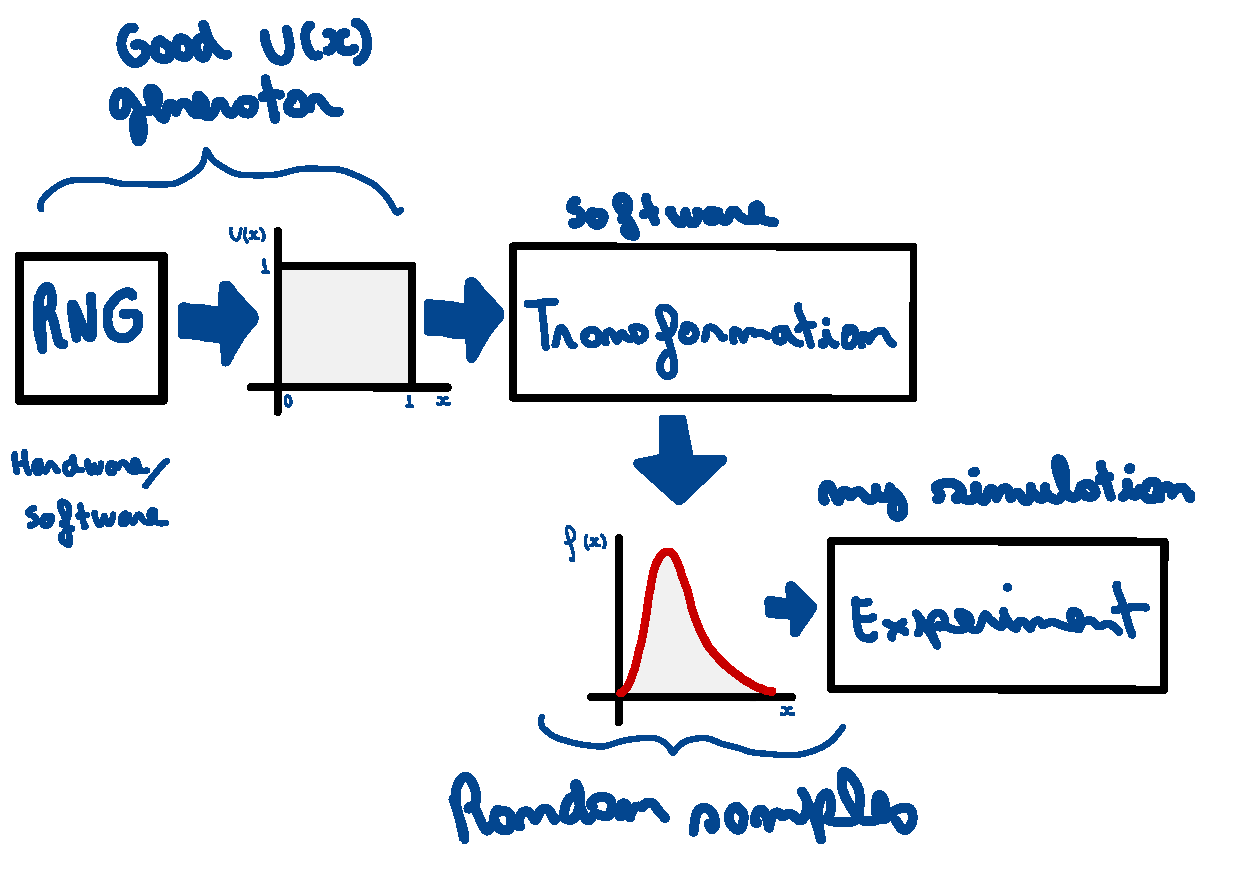
\includegraphics[width=0.95\textwidth]{sections/introduction/figures/simulation_framework.pdf}
    \end{figure}
\end{frame}







\section{Pseudo-Random Numbers Generators}


\begin{frame}
    \frametitle{Random Generators (RNG)}

    Our goal is to produce a sequence of random numbers in which number is
    independently drawn from the continuous uniform distribution on the interval
    $[0,1]$. There are two ways to generate a random number:

    \begin{itemize}

        \item \textbf{physical phenomenon of a random nature}, which can be slow and expensive;
        Classic examples: method of dernos that uses quantum effects, thermal noise in electrical circuits, 
        the radioactive decay, etc;

        \item \textbf{Pseudo-random numbers} generated by computer programs, which are fast and 
        reproducible, but always type determinisitcically and with apparently random output. 
   
    \end{itemize}
\end{frame}

\begin{frame}
    \frametitle{Pseudo-Random Number Generators (PRNG)}

    \begin{itemize}

        \item Refers to an algorithm that uses mathematical formulas to produce 
        sequences of random numbers;
        \item Starts from an arbitrary starting state using a \textbf{seed}; 

        \item \textbf{Efficient:} Can produce many numbers in a short time and is advantageous for 
        applications that need many numbers;

        \item \textbf{Deterministic:} A given sequence of numbers can be reproduced at a 
        later date if the starting point in the sequence is known.

        \item \textbf{Periodic:} Which means that the sequence will eventually repeat itself. 
        While periodicity is hardly ever a desirable characteristic, modern PRNGs have a period that is so long that it can be ignored for most practical purposes
    \end{itemize}
\end{frame}



\begin{frame}
    \frametitle{Linear Congruential Generator (LCG)}
    \begin{itemize}

        \item The method represents one of the oldest and best-known pseudorandom 
        number generator algorithms. Was \textbf{published in 1958} by W. E. Thomson and A. Rotenberg.
    
        $$Z_i = (aZ_{i-1}+c)(\text{mod} m)$$

        Where $i>=1$.
        
        \item To archieve appearance of randomness, the parameters $m$, $c$ and $a$ should be
        chosen to satisfy the following conditions:

        \begin{itemize}
            \item $a, c \geq 0$,
            \item $m > max(Z_0,a,c)$,
            \item $c$ and $m$ are relatively prime, i.e., they have no common divisor,
            \item $a-1$ is a multiple of 4 if $m$ is a multiple of 4, and
            \item $a-1$ is a multiple of $p$ for every prime $p$ that divides $m$.
        \end{itemize}
  
    \end{itemize}
\end{frame}

\begin{frame}
    \frametitle{Linear Congruential Generator (LCG)}
    \begin{figure}
        \centering
        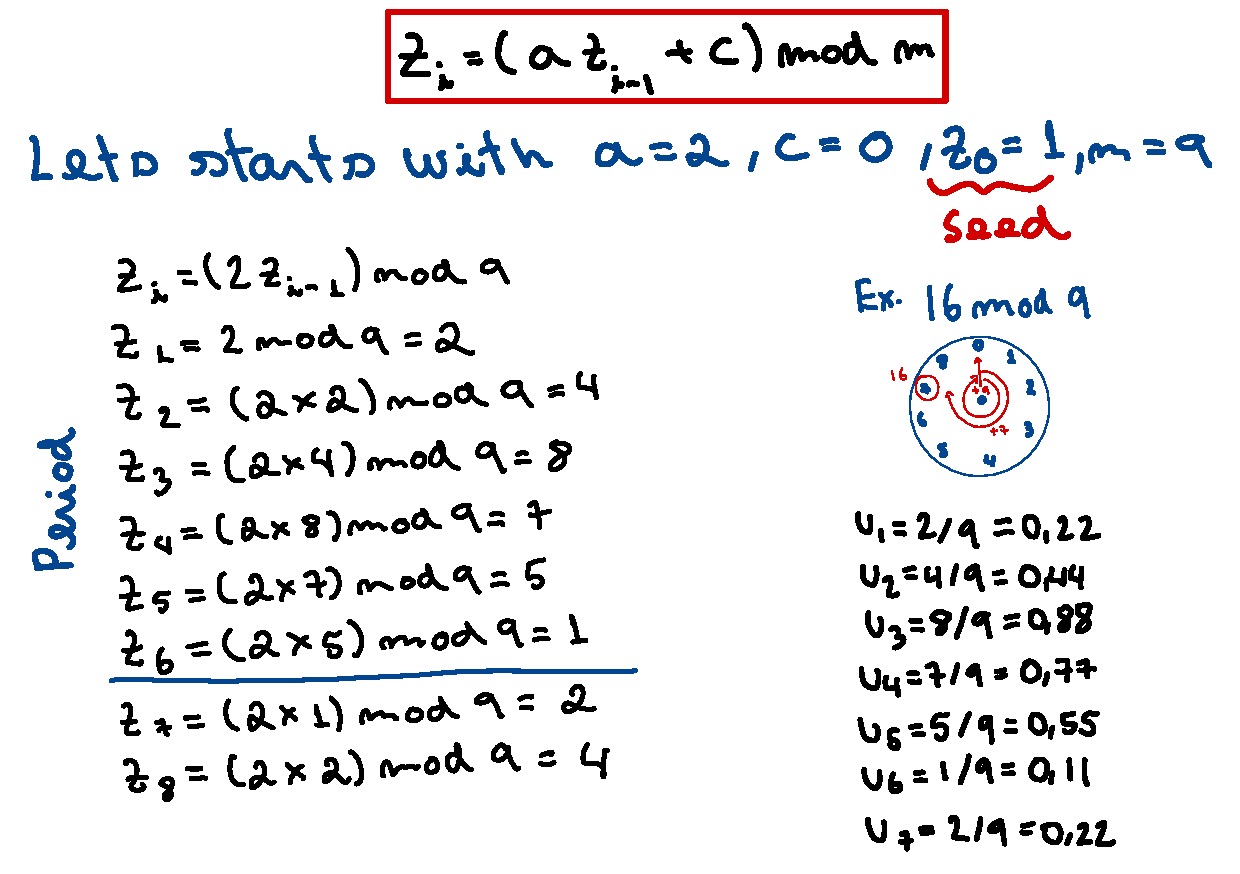
\includegraphics[width=0.95\textwidth]{sections/prng/figures/lcg_example.pdf}
    \end{figure}
\end{frame}

\begin{frame}
    \frametitle{Linear Congruential Generator (LCG)}
    
    \begin{itemize}
    \item In general, $m$ (circle table values) should be chosen as large as possible,
    since the period can never be longer than this.

    \item A good choice is the largest integer than can be represented on the computer. 
    For a 32-bit machine, the largest $m$ should be $2^{31}$.

    \item When $c$ is chosen to be zero, the algorithms reduces To

    $$Z_i = aZ_{i-1} \text{mod}m$$

    and is called the multiplicative congruent method (MCM) and is faster
    than LCG.

    \end{itemize}
\end{frame}



\begin{frame}
    \frametitle{Multiple Recursive Generators (MRGs)}
    
    \begin{itemize}
        \item Generalization of LCGs;

        \item Extended to incorporate not just the previous random integer (seed)
        into the formula, but a linear combination of the preceding random
        integers. For example, the sequence generated from:

        $$z_i = (a_1z_{i-1} _ a_2z_{i-2}) \text{mod} m$$
        
        \item It is common to use more than the two previousintegers to produce the 
        next sequence. The general form for MRGs should be:

        $$§z_i = \left(\sum_{j=1}^{k}a_jz_{i-j}\text{mod}m\right)$$

        Where it requires $k$ initial seeds, $z_0, z_1,...,z_{k-1}$.
    
    \end{itemize}
\end{frame}



\begin{frame}
    \frametitle{Mersenne Twister}
    
    \begin{itemize}

        \item \textbf{Developed in 1997} by Makoto Matsumoto and Takuji Nishimura. Its name 
        derives from the fact that its period length is chosen to be a Mersenne prime.

        \item Is one of the most extensively tested random number generators in existence. 
        However it is \textbf{completely unsuitable for cryptographic purposes}.

        \item \textbf{Python uses the Mersenne Twister} as the core generator. It produces 53-bit precision 
        floats and has a very long period of $2^{19937}-1$.

    \end{itemize}


\end{frame}


\begin{frame}
    \frametitle{Mersenne Twister}
    
    \begin{itemize}


    \end{itemize}


\end{frame}


\begin{frame}
    \frametitle{How to Build a Good Generator?}
    

    A consensus is building that even cycles of length are
    insufficient for current critical application such as cryptographic operations. How
    to build a good generator?

\end{frame}

\begin{frame}
    \frametitle{How to Build a Good Generator?}

    \begin{itemize}

        \item \textbf{Entropy input:} Combine a source of randomness from a physical process 
        to produce the initial state (seed) of a deterministic random generator.
        \begin{itemize}
            \item Desktops and server PCs can use four different sources of entropy: mouse
            and keyboard activity, disk I/O operations and specific interrupts;
            \item Cryptographic operations uses mode complex ones ((e.g. avalanche effect in zener diodo)
        \end{itemize}
        

    \end{itemize}
\end{frame}


\begin{frame}
    \frametitle{How to Build a Good Generator?}

    \begin{itemize}

        \item \textbf{Reseed Mechanism:} The reseed function acquires new entropy input and combines it with
        the current internal state and any additional input that is provided to create a new seed and a new
        internal state.
        
        \item \textbf{Deterministic robust algorithm}: For cryptographic operations, is used hash functions (e.g. HMAC) in order
        to produce pseudorandom bits.
        
        \item \textbf{Self-test}: Test function determines that the generator mechanism continues to 
        function correctly in order to ensure the quality.

    \end{itemize}
\end{frame}


\subsection{Validating Sequences of Random Numbers}

\begin{frame}
    \frametitle{Validating Sequences of Random Numbers}
    
    There are two approaches to testing random number generators:
    \begin{itemize}

        \item The empirical approach which involves running the generator many times and applying
        a series of statistical tests to evaluate the randomness of the generated sequence;

        \item And the mathematical analysis of the formulae upon which the generator is based (heavily on an undestating).

    \end{itemize}

    We will only consider the first approach.

\end{frame}



\begin{frame}
    \frametitle{Validating Sequences of Random Numbers}

    The empirical approches can be divided into two categories:

    \begin{itemize}

        \item Verify that the numbers in a given sequence are uniformly distributed over the interval [0,1). We shall
        consider in this category the \textit{chi-square goodness-of-fit test} and the \textit{Kolmogorov-Smirnov test}.

        \item Ensure that the numbers in the sequence are independent. We shall consider the \textit{run tests}, 
        a \textit{gap test} and the \textit{poker test}. 

    \end{itemize}


\end{frame}



\begin{frame}
    \frametitle{The \textit{Chi-square Goodness-of-fit} Test}
    
    \begin{itemize}

        \item Allow us to compare a sample distribution against a theoretical one;

        \item In our case, we would line to check just how uniformly a particular sequence
        of random numbers is distributed;


        \item To proceed, we partition an interval containing $n$ pseudorandom numbers into 
        $k$ equal subintervals (\textit{bins}) and compare the count of random numbers in 
        each \textit{bin} to the theoretical count of $n/k$.

        \item In other words, compare two histograms;
    
    \end{itemize}


\end{frame}


\begin{frame}
    \frametitle{The \textit{Chi-square Goodness-of-fit} Test}
    
    \begin{itemize}

        \item Compute the chi-square, $\chi^2$ to measure the degree of similarity of two
        probability mass functions ($pdfs$):

        $$\chi^2 = \sum_{i=1}^k\frac{(n_i - \bar{n_i})^2}{\bar{n_i}}$$
    
        Where $n_i$ is the count number inside of the \textit{bin} (experiment) and 
        $\bar{n_i} - n/k$ for all $i$ (theoretical).

        \item Perform the hypothesis test, i.e., the null hypothesis, must be accepted if the computed
        $\chi^2$ is less than the value $\chi_{\alpha}^2$ obtained from the table.


    \end{itemize}


\end{frame}


\begin{frame}
    \frametitle{The \textit{Chi-square Goodness-of-fit} Test}
    \begin{figure}
        \centering
        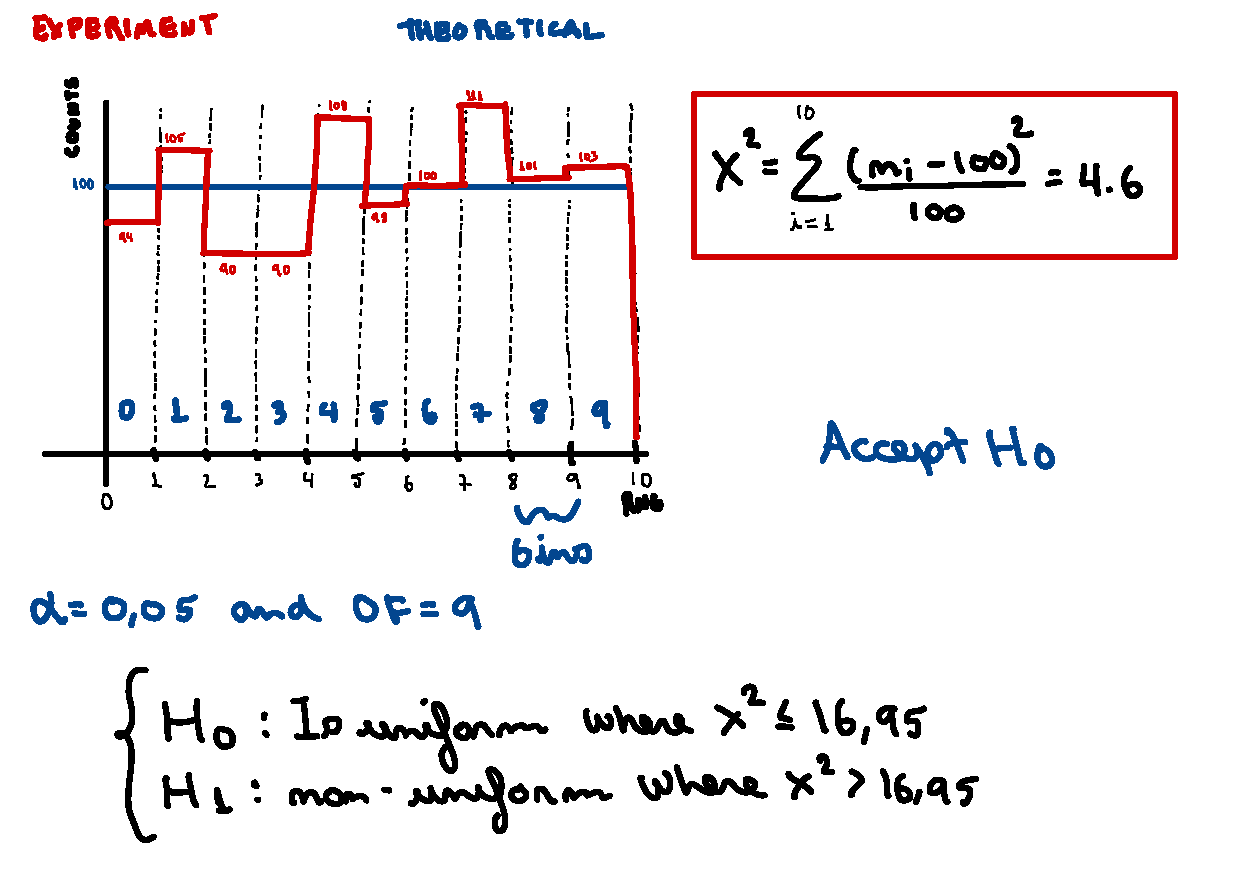
\includegraphics[width=0.95\textwidth]{sections/prng/figures/chi2_example.pdf}
    \end{figure}
\end{frame}



\begin{frame}
    \frametitle{The \textit{Kolmogorov-Smirnov Test}}

    Quantifies a distance between the empirical distribution function (experiment)
    and the cumulative distribution function of the reference (theoretical);
    \begin{itemize}
 
        \item Generate a set of $N$ random numbers $z_1,z_2,...,z_n$ in the interval [0,1)
        and arrange then into a nondecreasing order;

        \item Compute the quantities for $i \in [1,N]$:

        $$D^+=max\left(\frac{i}{N}-z_i\right), D^-=max\left(z_i-\frac{i-1}{N}\right)$$
        $$D=max(D^+,D^-)$$

        \item Consult tables of KS critical values and choose the $D_{\alpha}$
        \item If $D\leq D_{\alpha}$ accept the hypothesis that the numbers are
        uniformly distributed.


    \end{itemize}

\end{frame}

\begin{frame}
    \frametitle{The \textit{Kolmogorov-Smirnov Test}}
    \begin{figure}
        \centering
        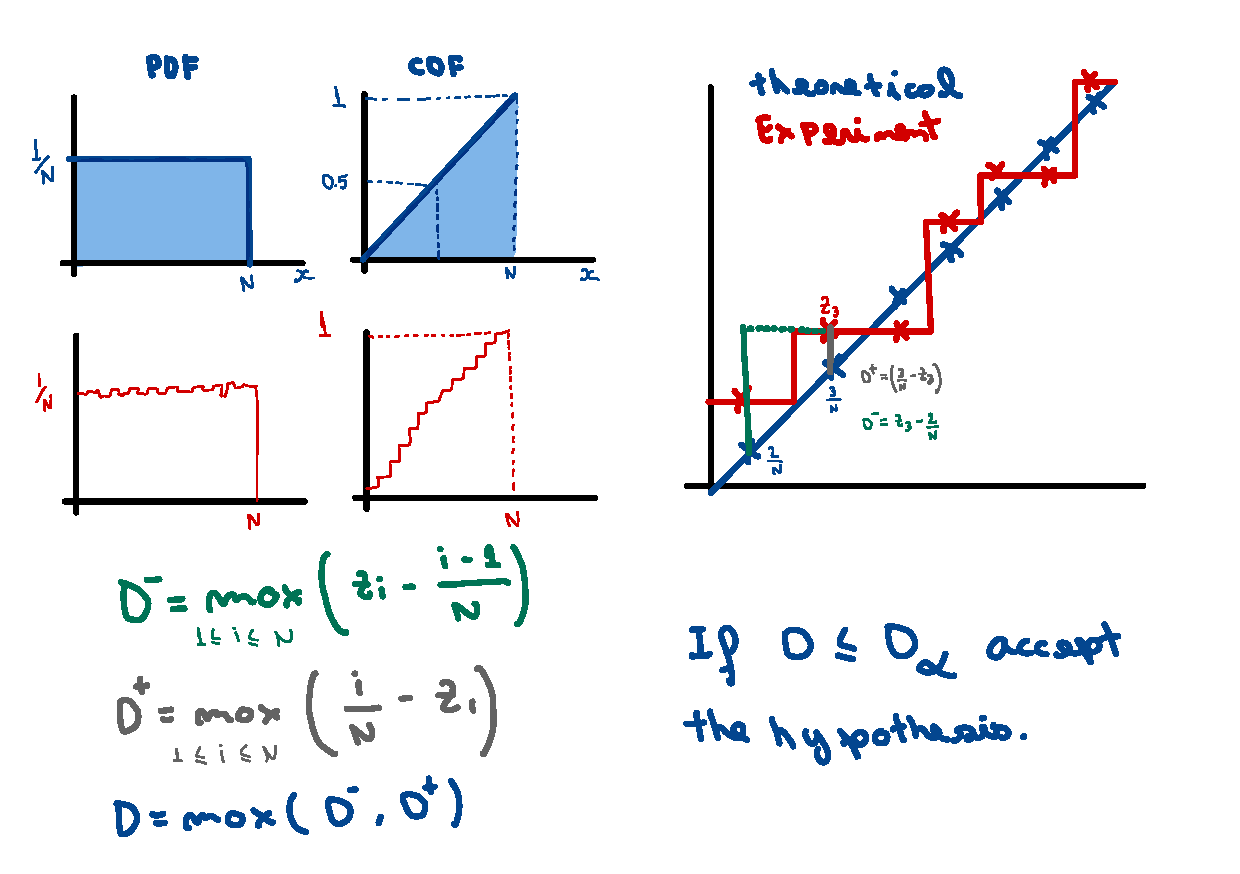
\includegraphics[width=0.95\textwidth]{sections/prng/figures/ks_example.pdf}
    \end{figure}
\end{frame}


\begin{frame}
    \frametitle{Run tests}

    \begin{itemize}
        \item The chi-square and Kolmogorov-Smirnov tests may be used to test the distribution
        of randomly generated numbers (experiment) against a given distribution (theoretical).

        \item However, they do not provide us with any information concerning the independence
        of the generated numbers.

        \item \textbf{\textit{Run} tests}: The total number of runs, runs above or below the mean and 
        the distribution of Run-ups (or Run-downs)

    \end{itemize}

\end{frame}




\begin{frame}
    \frametitle{Run tests}
    Given a sequence of random numbers, let's define:

    \begin{itemize}
        \item A \textit{run-up} in a sequence of numbers is a subsequence
        in which each successive number is greater than the previous;

        \item A \textit{run-down} is a subsequence with the opposite property.
    \end{itemize}
\end{frame}



\begin{frame}
    \frametitle{Run tests: The total number of runs}
    Given a sequence of random numbers, let's define:

    \begin{itemize}
        \item A \textit{run-up} in a sequence of numbers is a subsequence
        in which each successive number is greater than the previous;

        \item A \textit{run-down} is a subsequence with the opposite property.
    \end{itemize}
\end{frame}

\subsection{Statistical Test Suites}

\begin{frame}
    \frametitle{Statistical Test Suites}

    \begin{itemize}
       
        \item For critical operations (e.g. Hardware security modules, cryptographic operations, 
        electronic vote machine) it is necessary to implement a approved random generator;

        \item Random generators (e.g. DRBG) are specified 
        by \href{https://csrc.nist.gov/publications/detail/sp/800-90a/rev-1/final}{SP 800-90A} from NIST;

        \item Two suites of renown are the \href{https://github.com/arcetri/sts}{NIST} (National Intitute 
        of Standards and Technology) which contains a collection of 16 tests 
        and the \href{https://github.com/GINARTeam/Diehard-statistical-test}{DIEHARD} with 12 tests. For critical operations, the PRNG must be
        approved in all tests;

        \item NIST recommends that $\alpha$ be in the range $[0.001, 0.01]$.

    \end{itemize}
\end{frame}


\section{Nonuniformly Distributed Random Numbers}

\begin{frame}
    \frametitle{Nonuniformly Distributed Random Numbers}

    \begin{itemize}

        \item In simulation, the distribution of the occurrence of events
        is numbers that are perhaps exponentially distributed or normally
        distributed or have some other appropriate distribution;

        \item This is accomplished by generating a sequence of uniformly distributed 
        random numbers and transforming this sequence to a sequence having
        the required distribution;

        \item To performing this transformation, we can use \textbf{the inverse transformation
        method}.
       

    \end{itemize}
\end{frame}


\begin{frame}
    \frametitle{Nonuniformly Distributed Random Numbers}
    \begin{figure}
        \centering
        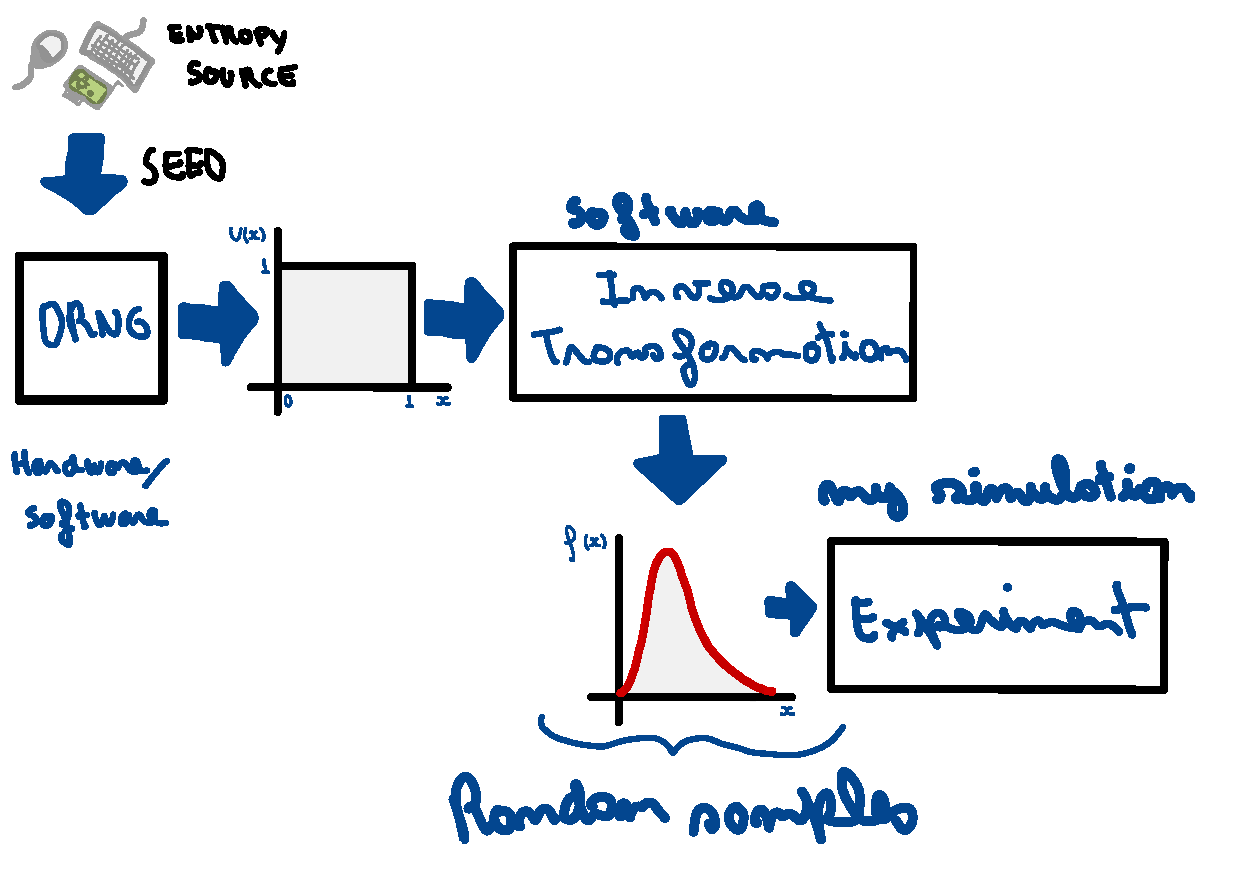
\includegraphics[width=0.95\textwidth]{sections/prng/figures/simulation_framework_plus.pdf}
    \end{figure}
\end{frame}

\subsection{Inverse Transform}

\begin{frame}
    \frametitle{Inverse Transform}
    
    \begin{itemize}

        \item Can be used when the distribution function can be analytically inverted;

        \item The $F(x)$ (cumulative distrbution function) has a value that lies 
        between 0 and 1, just like our uniformly distrubuted random numbers;

        \item First, generate a number $u_i$ between o and 1 
        (from a uniform distribution, e.g. PRNG) and then
        find the corresponding $x_i$ coordinate by using $F^{-1}$;

        \item For various values of $u_i$, the $x_i$ will 
        be properly distributed along the x-axis;

        \item It is one-to-one mapping between $u_i$ and $x_i$ along the $F(x)$ curve.
    \end{itemize}
\end{frame}



\begin{frame}
    \frametitle{Inverse Transform}
    \begin{figure}
        \centering
        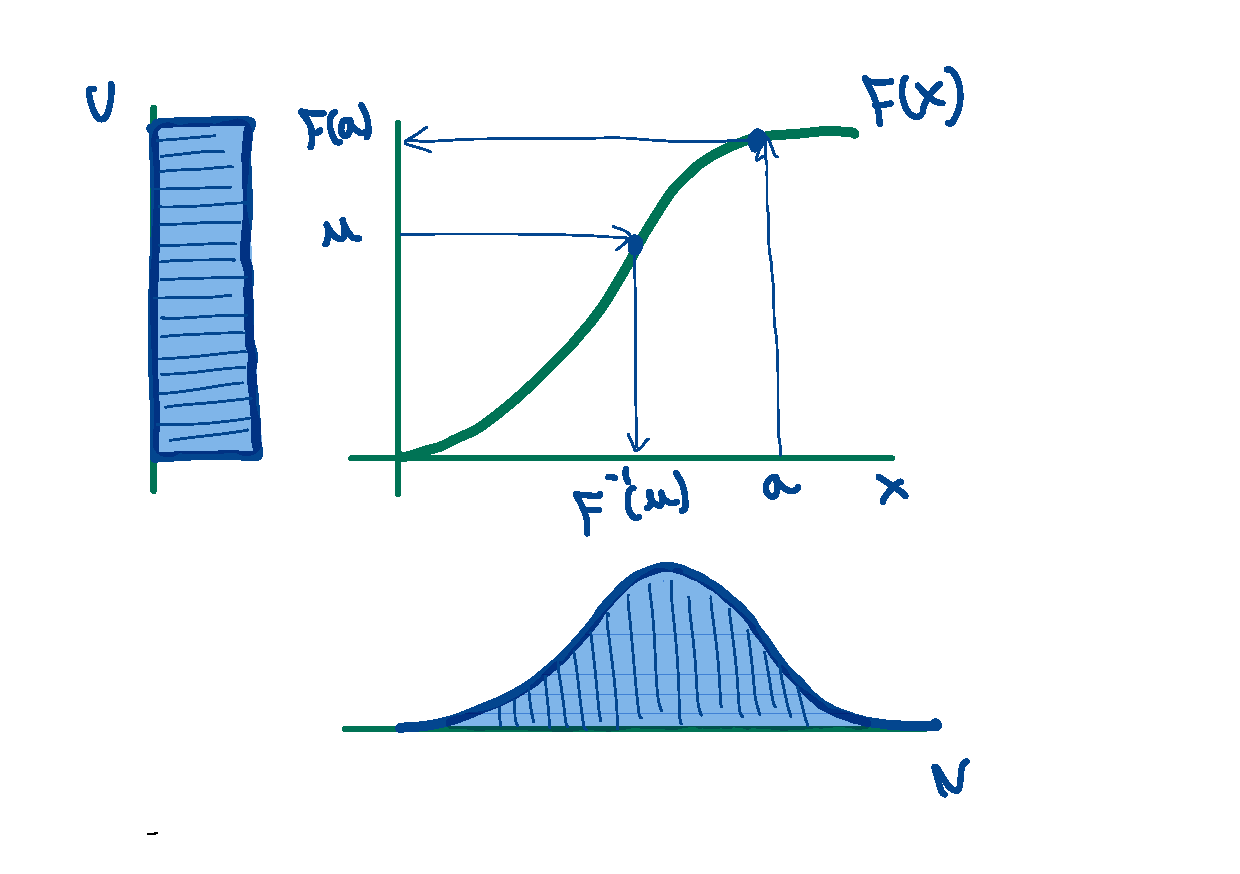
\includegraphics[width=0.95\textwidth]{sections/prng/figures/inverse_method_continuous.pdf}
    \end{figure}
\end{frame}


\begin{frame}
    \frametitle{Inverse Transform}
    
    No discrete distribution function can be inverted, since such a function
    is a stepwise function rather than one that is strictly increasing. But, in such cases,
    it still possible to use the invertion approache.

    \begin{figure}
        \centering
        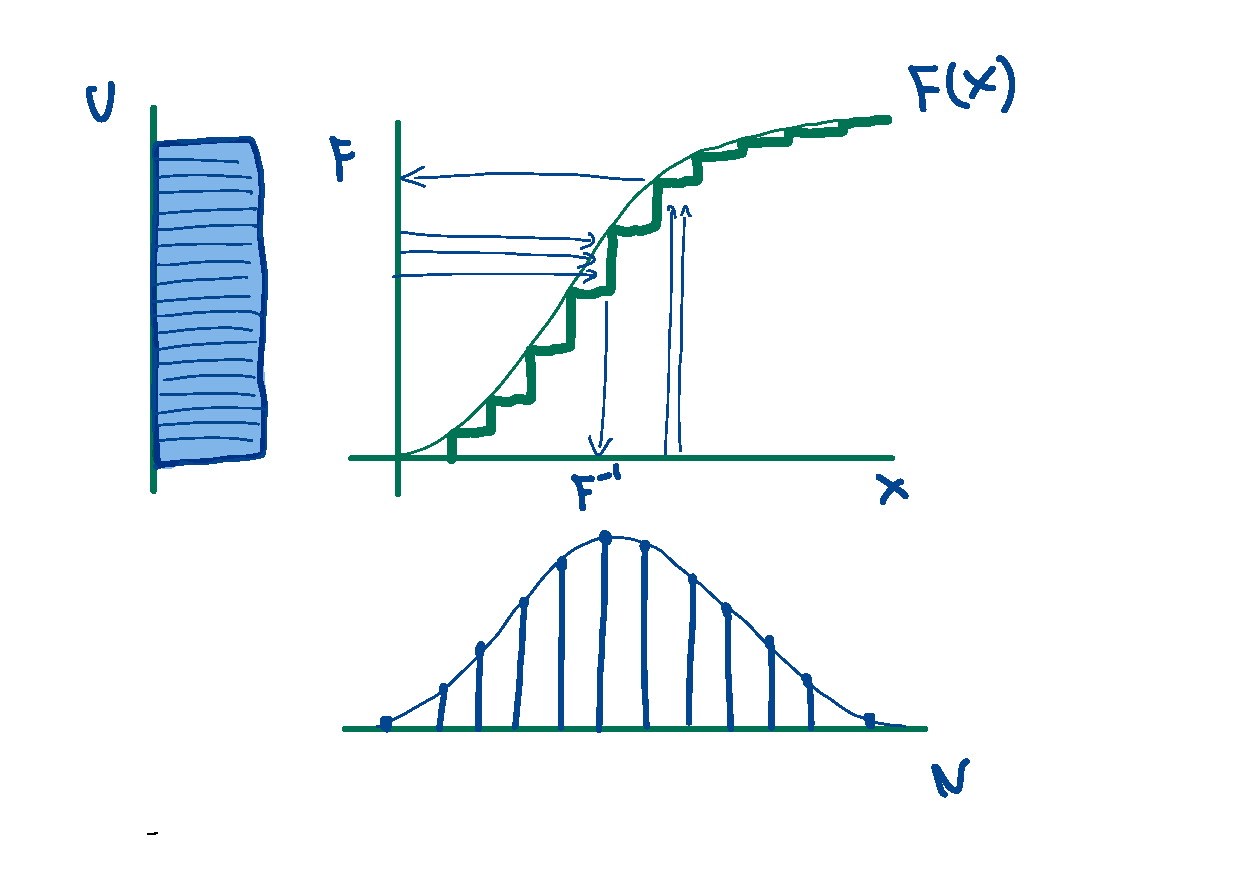
\includegraphics[width=0.7\textwidth]{sections/prng/figures/inverse_method_discrete.pdf}
    \end{figure}


\end{frame}



\begin{frame}
    \frametitle{Inverse Transform: The Continuous Uniform Distribution}
    The probability density and cumulative distribution functions for continuous random variables that
    are uniformly distribution on the interval $[a,b]$ are respectively given by
    \begin{figure}
        \centering
        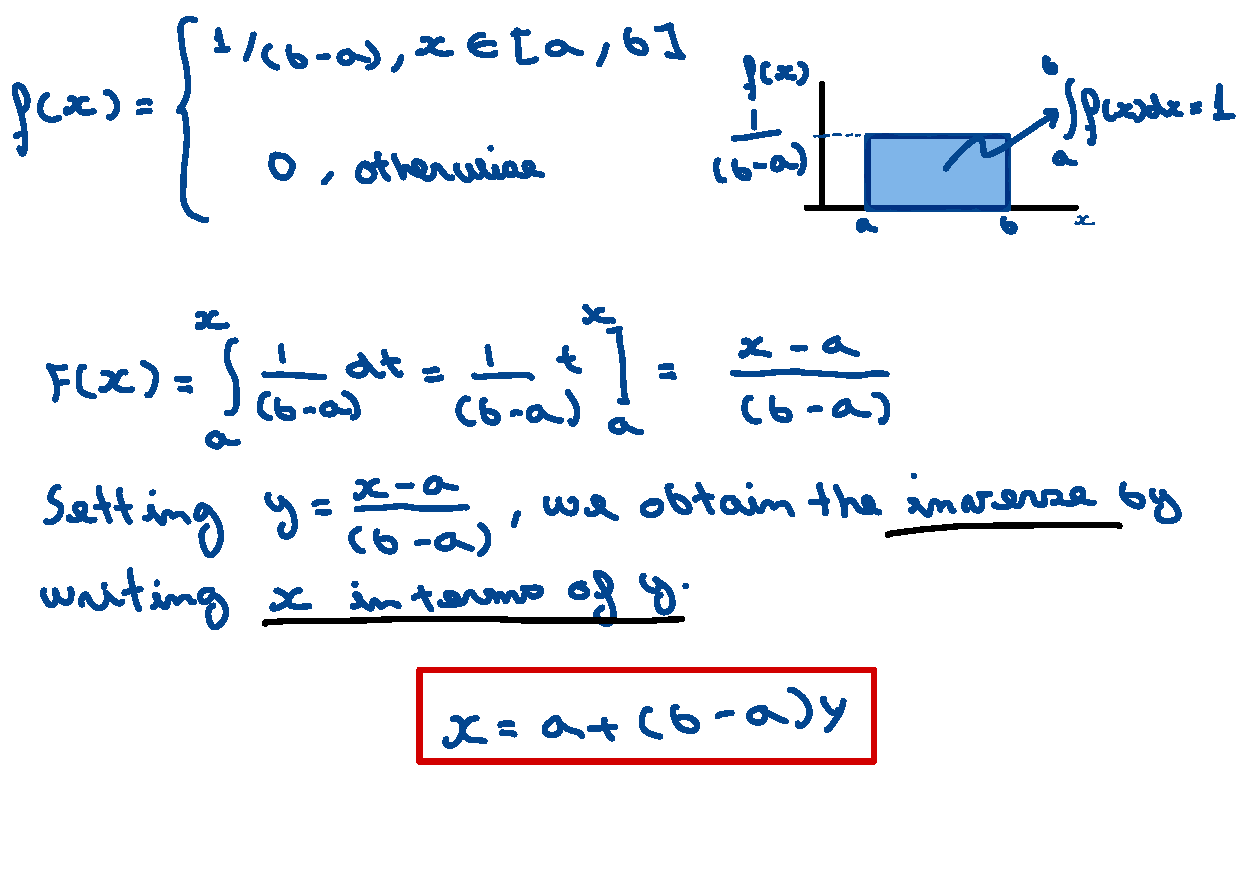
\includegraphics[width=0.8\textwidth]{sections/prng/figures/uniform_dist_example.pdf}
    \end{figure}
\end{frame}



\begin{frame}
    \frametitle{Inverse Transform: Wedge Shaped Functions}
    
    \begin{figure}
        \centering
        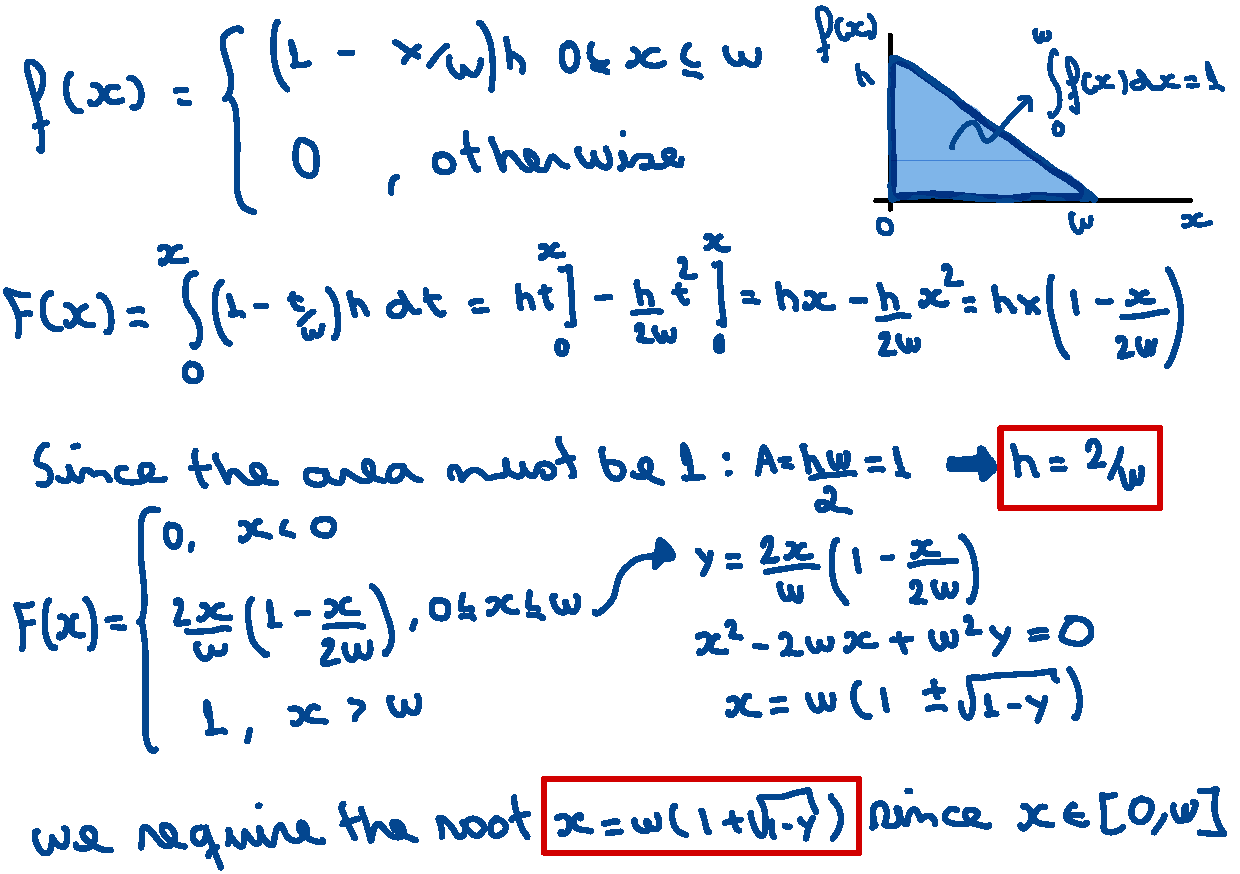
\includegraphics[width=0.9\textwidth]{sections/prng/figures/wedge_shaped_example.pdf}
    \end{figure}
\end{frame}


\begin{frame}
    \frametitle{Inverse Transform: Triangular Density Functions}
    
    \begin{figure}
        \centering
        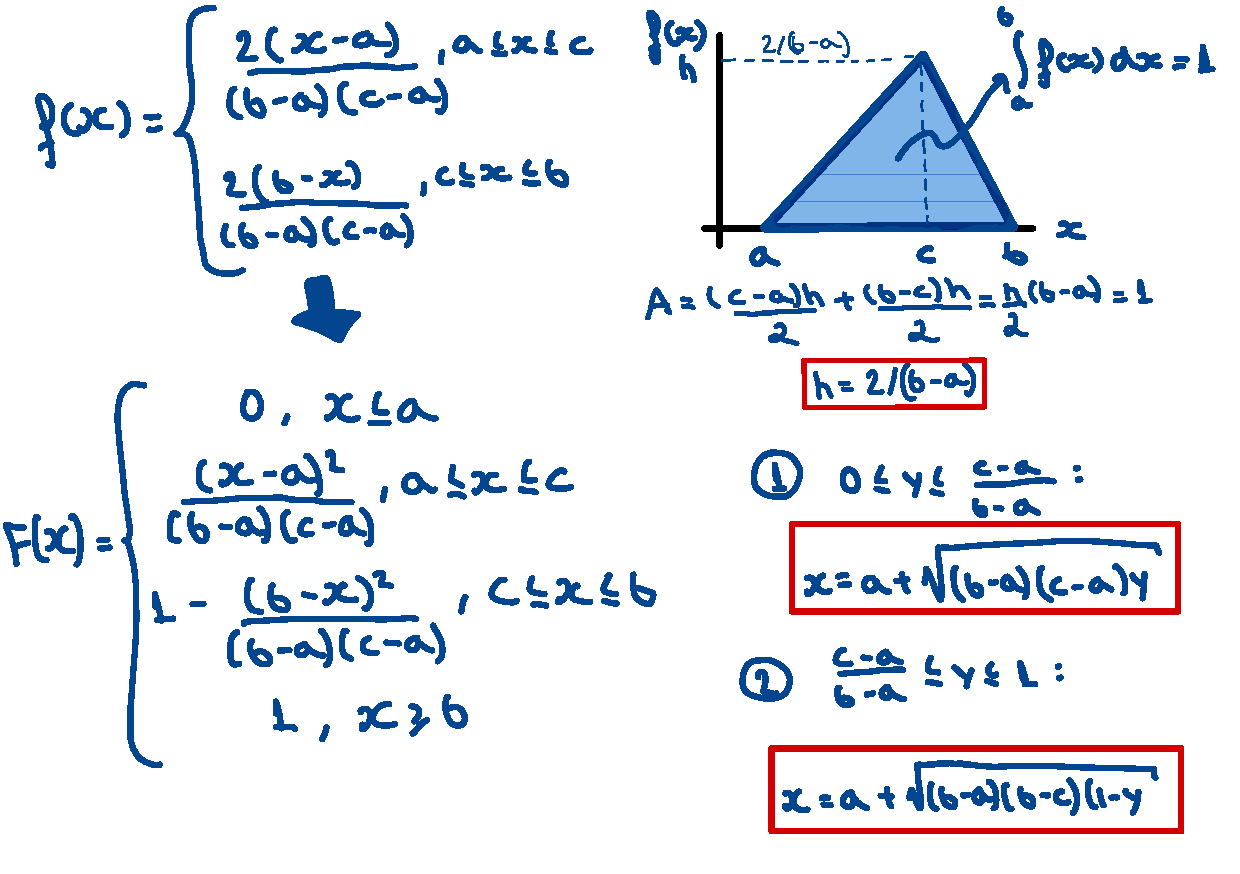
\includegraphics[width=0.9\textwidth]{sections/prng/figures/triangular_dist_example.pdf}
    \end{figure}
\end{frame}

\begin{frame}
    \frametitle{Inverse Transform: Exponential Distribution}
    \begin{figure}
        \centering
        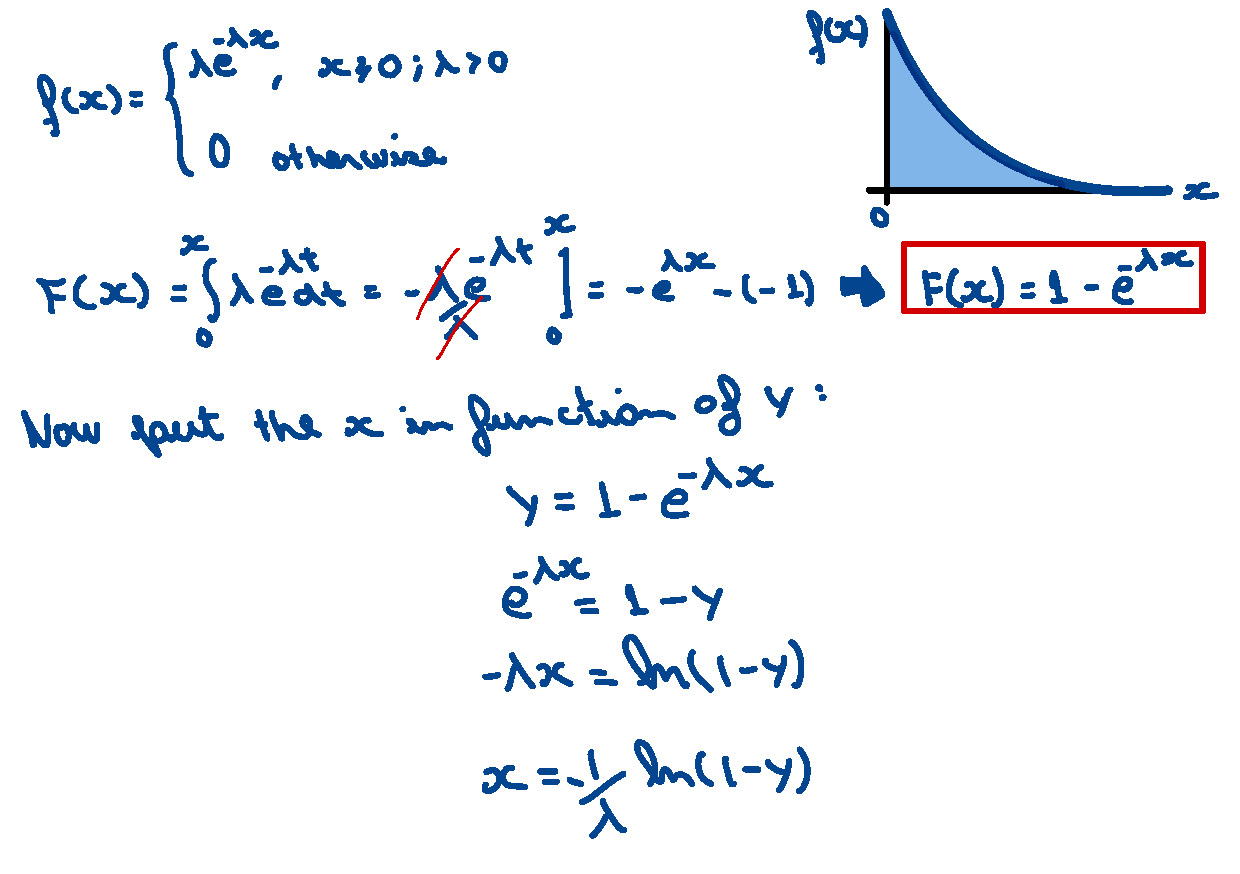
\includegraphics[width=0.9\textwidth]{sections/prng/figures/exp_dist_example.pdf}
    \end{figure}
\end{frame}


\begin{frame}
    \frametitle{Inverse Transform: An Arbitrary Discrete Distribution}
    \begin{itemize}

        \item Consider a more general case of a random variable havind a discrete probability mass
        function and probability distribution function:

        $$p(x_i) = P(X=x_i) \text{and} F(x) = P(X\leq x)$$

        \item As we mentioned before, a number that falls in the \textit{bin} $[F(x_{x-1}), F(x_i)]$
        is associated with the event $X=x_i$

        \item The general case is used when we don't know the mathematical formulation of the density function.

        \item We can measure a lot of real events (e.g. from the nature) to build the histogram 
        and estimate the approximated distribution.

        \item This estimated distributiton can be used to simulate new events based on the real data.
    \end{itemize}

\end{frame}



\begin{frame}
    \frametitle{Inverse Transform: An Arbitrary Discrete Distribution}
    \begin{figure}
        \centering
        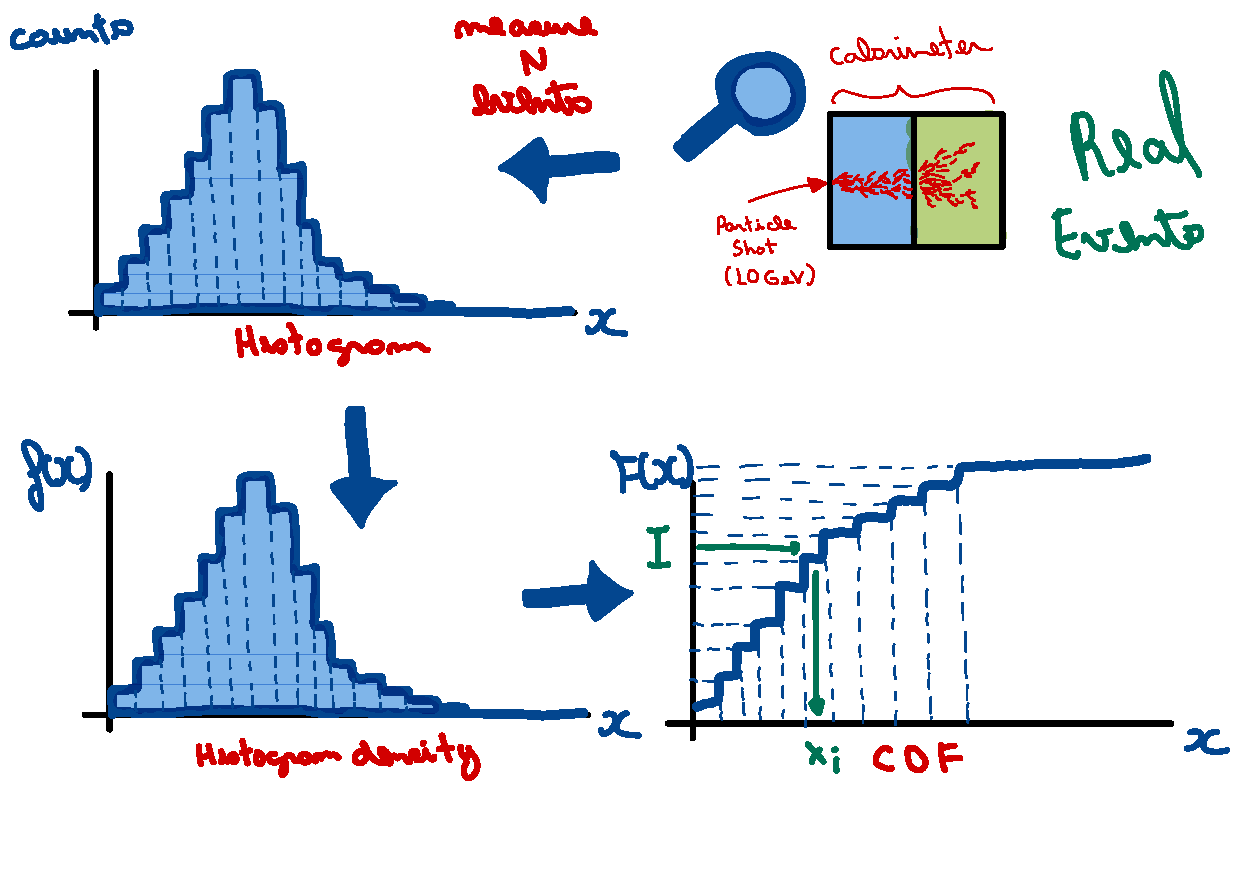
\includegraphics[width=0.9\textwidth]{sections/prng/figures/real_to_sim.pdf}
    \end{figure}
\end{frame}




\section{Simulation}

\begin{frame}
    \frametitle{Simulation}

    Until here, we learned about PRNGs and how to transform a uniformly distribution
    into others. Now, let's talk about event simulation.

\end{frame}


\end{document}